% THIS DOCUMENT IS FOLLOWS THE VOLERE TEMPLATE BY Suzanne Robertson and James Robertson
% ONLY THE SECTION HEADINGS ARE PROVIDED
%
% Initial draft from https://github.com/Dieblich/volere
%
% Risks are removed because they are covered by the Hazard Analysis
\documentclass[12pt]{article}

\usepackage{booktabs}
\usepackage{tabularx}
\usepackage{longtable}
\usepackage{graphicx}
\usepackage{hyperref}
\usepackage{float}
\graphicspath{ {./res/} }
\hypersetup{
    bookmarks=true,         % show bookmarks bar?
      colorlinks=true,      % false: boxed links; true: colored links
    linkcolor=red,          % color of internal links (change box color with linkbordercolor)
    citecolor=green,        % color of links to bibliography
    filecolor=magenta,      % color of file links
    urlcolor=cyan           % color of external links
}

\newcommand{\lips}{\textit{Insert your content here.}}

%% Comments

\usepackage{color}

\newif\ifcomments\commentstrue %displays comments
%\newif\ifcomments\commentsfalse %so that comments do not display

\ifcomments
\newcommand{\authornote}[3]{\textcolor{#1}{[#3 ---#2]}}
\newcommand{\todo}[1]{\textcolor{red}{[TODO: #1]}}
\else
\newcommand{\authornote}[3]{}
\newcommand{\todo}[1]{}
\fi

\newcommand{\wss}[1]{\authornote{blue}{SS}{#1}} 
\newcommand{\plt}[1]{\authornote{magenta}{TPLT}{#1}} %For explanation of the template
\newcommand{\an}[1]{\authornote{cyan}{Author}{#1}}

%% Common Parts

\newcommand{\progname}{ProgName} % PUT YOUR PROGRAM NAME HERE
\newcommand{\authname}{Team \#, Team Name
\\ Student 1 name
\\ Student 2 name
\\ Student 3 name
\\ Student 4 name} % AUTHOR NAMES                  

\usepackage{hyperref}
    \hypersetup{colorlinks=true, linkcolor=blue, citecolor=blue, filecolor=blue,
                urlcolor=blue, unicode=false}
    \urlstyle{same}
                                


\begin{document}

\title{Software Requirements Specification for \progname: subtitle describing software} 
\author{\authname}
\date{\today}
	
\maketitle

~\newpage

\pagenumbering{roman}

\tableofcontents

~\newpage

\section*{Revision History}

\begin{tabularx}{\textwidth}{p{3cm}p{2cm}X}
\toprule {\textbf{Date}} & {\textbf{Version}} & {\textbf{Notes}}\\
\midrule
Date 1 & 1.0 & Notes\\
Date 2 & 1.1 & Notes\\
\bottomrule
\end{tabularx}

~\\

~\newpage
\section{Purpose of the Project}
\subsection{User Business}

With the world currently facing record high inflation, cost-of-living is at the highest
it has ever been. This affects all daily necessities but is especially true for food and groceries.
As a whole, all households are affected but there is particular financial strain on those with lower-incomes.
As a result, interest in personal finance has grown and become more important in peoples' everyday lives.
To assist these individuals, we are developing an application that can help users better understand their
spending habits and make smarter financial decisions. This application will allow users to
take photos of grocery receipts and track their overall spending, analyze spending trends, and receive
suggestions on cheaper alternatives for purchased grocery items. Overall, we believe this application
will help users stay more informed and reduce grocery spending in the long-term.

\subsection{Goals of the Project}
\begin{itemize}
  \item The created application will help users save money on groceries over time.
  \item The application will provide accurate spending data and suggestions to end users.
\end{itemize}  
\section{Stakeholders}
\subsection{Client}
\lips
\subsection{Customer}
\lips
\subsection{Other Stakeholders}
\lips
\subsection{Hands-On Users of the Project}
\lips
\subsection{Personas}
\lips
\subsection{Priorities Assigned to Users}
\lips
\subsection{User Participation}
\lips
\subsection{Maintenance Users and Service Technicians}
\lips

\section{Mandated Constraints}
\subsection{Solution Constraints}
\lips
\subsection{Implementation Environment of the Current System}
\lips
\subsection{Partner or Collaborative Applications}
\lips
\subsection{Off-the-Shelf Software}
\lips
\subsection{Anticipated Workplace Environment}
\lips
\subsection{Schedule Constraints}
\lips
\subsection{Budget Constraints}
\lips
\subsection{Enterprise Constraints}
\lips

\section{Naming Conventions and Terminology}
\subsection{Glossary of All Terms, Including Acronyms, Used by Stakeholders
involved in the Project}
\lips

\section{Relevant Facts And Assumptions}
\subsection{Relevant Facts}
\lips
\subsection{Business Rules}
\lips
\subsection{Assumptions}
\lips

\section{The Scope of the Work}
\subsection{The Current Situation}
\lips
\subsection{The Context of the Work}
\lips
\subsection{Work Partitioning}
\lips
\subsection{Specifying a Business Use Case (BUC)}
\lips

\section{Business Data Model and Data Dictionary}
\subsection{Business Data Model}
\begin{figure}[H]
    \centering
    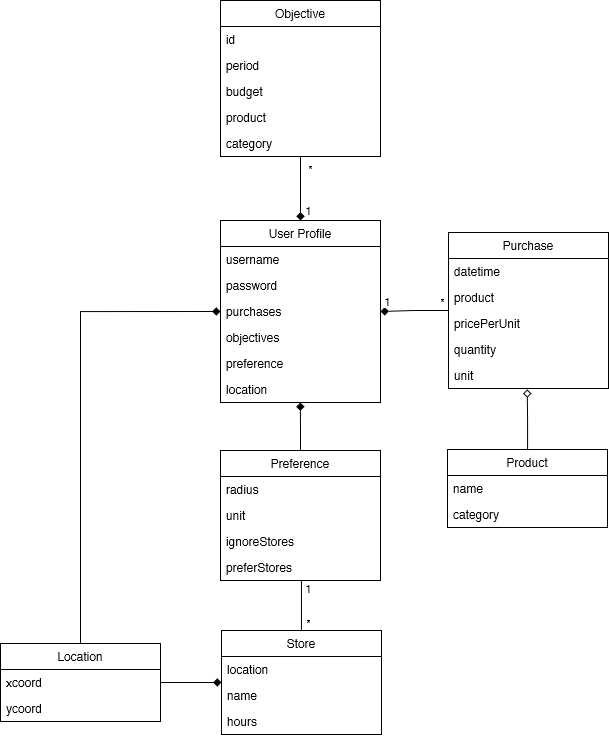
\includegraphics[width=0.85\textwidth]{classdiagram}
    \caption{Class Diagram}
    \label{fig:classdiagram}
\end{figure}
\subsection{Data Dictionary}
\begin{longtable}{| >{\raggedright\arraybackslash}p{.20\textwidth} | >{\raggedright\arraybackslash}p{.55\textwidth} | >{\raggedright\arraybackslash}p{.15\textwidth} |}
        \hline
        \textbf{Name} & \textbf{Content} & \textbf{Type} \\
        \hline
        User Profile & Username + Password + Purchases + Objectives + User Preference + User Location & Class \\
        \hline
        Objective & Objective Id + Period + Budget + Target Product + Target Category & Class \\
        \hline
        Purchase & Datetime + Purchased Product + Price Per Unit + Quantity + Unit & Class \\
        \hline
        Product & Product Name + Category & Class \\
        \hline
        Preference & Accessible Radius + Ignore Stores + Prefer Stores + Prefer Units & Class \\
        \hline
        Store & Store Location + Store Name & Class \\
        \hline
        Location & X-Coordinate + Y-Coordinate & Class \\
        \hline
        Username & *Unique String* & Attribute\\
        \hline
        Password & *String* & Attribute \\
        \hline
        Purchases & *List of Purchase class* & Attribute \\
        \hline
        Objectives & *List of Objective class* & Attribute \\
        \hline
        User Preference & *Preference class* & Attribute \\
        \hline
        User Location & *Location class* & Attribute \\
        \hline
        Objective Id & *String* & Attribute \\
        \hline
        Period & *String: day/week/month/year* & Attribute\\
        \hline
        Budget & *Currency amount measured by Double to 2 decimals* & Attribute \\
        \hline
        Target Product & *String product name* & Attribute \\
        \hline 
        Target Category & *String category name* & Attribute \\
        \hline 
        Datetime & *YYYY-MM-DD HH:MM:SS* & Attribute \\
        \hline 
        Purchased Product & *String Product name* & Attribute \\
        \hline 
        Price Per Unit & *Int price per unit of product* & Attribute \\
        \hline 
        Unit & *String* & Attribute \\
        \hline 
        Quantity & *Double* & Attribute \\
        \hline 
        Product Name & *String* & Attribute \\
        \hline 
        Category & *String* & Attribute \\
        \hline 
        Accessible Radius & *Integer* & Attribute \\
        \hline 
        Ignore Stores & *List of Stores to ignore* & Attribute \\
        \hline 
        Prefer Stores & *List of Stores to prioritise* & Attribute \\
        \hline 
        Prefer Units & *String: metric/imperial* & Attribute \\
        \hline
        Store Location & *Location class* & Attribute \\
        \hline 
        Store Name & *String* & Attribute \\
        \hline 
        X Coordinate & *Double* & Attribute \\
        \hline 
        Y Coordinate & *Double* & Attribute \\
        \hline 
        \caption{Business Event List}
        \label{tab:businesseventlist}
    \end{longtable}

\section{The Scope of the Product}
\subsection{Product Boundary}
\lips
\subsection{Product Use Case Table}
\lips
\subsection{Individual Product Use Cases (PUC's)}
\lips

\section{Functional Requirements}
\subsection{Functional Requirements}
\lips

\section{Look and Feel Requirements}
\subsection{Appearance Requirements}
\lips
\subsection{Style Requirements}
\lips

\section{Usability and Humanity Requirements}
\subsection{Ease of Use Requirements}
\lips
\subsection{Personalization and Internationalization Requirements}
\lips
\subsection{Learning Requirements}
\lips
\subsection{Understandability and Politeness Requirements}
\lips
\subsection{Accessibility Requirements}
\lips

\section{Performance Requirements}
\subsection{Speed and Latency Requirements}
\lips
\subsection{Safety-Critical Requirements}
\lips
\subsection{Precision or Accuracy Requirements}
\lips
\subsection{Robustness or Fault-Tolerance Requirements}
\lips
\subsection{Capacity Requirements}
\lips
\subsection{Scalability or Extensibility Requirements}
\lips
\subsection{Longevity Requirements}
\lips

\section{Operational and Environmental Requirements}
\subsection{Expected Physical Environment}
\lips
\subsection{Wider Environment Requirements}
\lips
\subsection{Requirements for Interfacing with Adjacent Systems}
\lips
\subsection{Productization Requirements}
\lips
\subsection{Release Requirements}
\lips

\section{Maintainability and Support Requirements}
\subsection{Maintenance Requirements}
\lips
\subsection{Supportability Requirements}
\lips
\subsection{Adaptability Requirements}
\lips

\section{Security Requirements}
\subsection{Access Requirements}
\lips
\subsection{Integrity Requirements}
\lips
\subsection{Privacy Requirements}
\lips
\subsection{Audit Requirements}
\lips
\subsection{Immunity Requirements}
\lips

\section{Cultural Requirements}
\subsection{Cultural Requirements}
\lips

\section{Compliance Requirements}
\subsection{Legal Requirements}
\lips
\subsection{Standards Compliance Requirements}
\lips

\section{Open Issues}
\lips

\section{Off-the-Shelf Solutions}
\subsection{Ready-Made Products}
\lips
\subsection{Reusable Components}
\lips
\subsection{Products That Can Be Copied}
\lips

\section{New Problems}
\subsection{Effects on the Current Environment}
\lips
\subsection{Effects on the Installed Systems}
\lips
\subsection{Potential User Problems}
\lips
\subsection{Limitations in the Anticipated Implementation Environment That May
Inhibit the New Product}
\lips
\subsection{Follow-Up Problems}
\lips

\section{Tasks}
\subsection{Project Planning}
\lips
\subsection{Planning of the Development Phases}
\lips

\section{Migration to the New Product}
\subsection{Requirements for Migration to the New Product}
\lips
\subsection{Data That Has to be Modified or Translated for the New System}
\lips

\section{Costs}
\lips
\section{User Documentation and Training}
\subsection{User Documentation Requirements}
\lips
\subsection{Training Requirements}
\lips

\section{Waiting Room}
\lips

\section{Ideas for Solution}
\lips

\newpage{}
\section*{Appendix --- Reflection}

The information in this section will be used to evaluate the team members on the
graduate attribute of Lifelong Learning.  Please answer the following questions:

\begin{enumerate}
  \item What knowledge and skills will the team collectively need to acquire to
  successfully complete this capstone project?  Examples of possible knowledge
  to acquire include domain specific knowledge from the domain of your
  application, or software engineering knowledge, mechatronics knowledge or
  computer science knowledge.  Skills may be related to technology, or writing,
  or presentation, or team management, etc.  You should look to identify at
  least one item for each team member.
  \item For each of the knowledge areas and skills identified in the previous
  question, what are at least two approaches to acquiring the knowledge or
  mastering the skill?  Of the identified approaches, which will each team
  member pursue, and why did they make this choice?
\end{enumerate}

\end{document}